\documentclass[a4paper,12pt,]{report}
%\documentclass[a4paper,12pt,landscape,twocolumn]{report}
\usepackage[a4paper, inner=1.7cm, outer=2.7cm, top=2cm, bottom=2cm,bindingoffset=1.2cm ]{geometry}

% \renewcommand{\familydefault}{\sfdefault}
\usepackage[english]{babel}

\usepackage{blindtext}
\usepackage[scaled=.92]{helvet}

\usepackage{microtype}
\usepackage{graphicx}
\usepackage{wrapfig}
\usepackage{enumitem}
\usepackage{fancyhdr}
\usepackage{amsmath}
\usepackage{index}

% \usepackage[onehalfspacing]{setspace}

\newcommand{\NTT}{New Think Tank}
\newcommand{\NTTB}{\textbf{New Think Tank}}
\newcommand{\typew}[1]{\texttt{#1}}


\pagestyle{fancy}


\makeindex

\begin{document}
\title{\Large{\textbf{LaTex Practice}}}
\author{Mortos der Soulstealer}
\date{31.07.2019}

\maketitle

\tableofcontents

\pagenumbering{roman}
\setcounter{page}{2}

\fancyhf{}
\renewcommand{\headrulewidth}{2pt}
\renewcommand{\footrulewidth}{2pt}

\fancyhead[LE]{\leftmark}
\fancyhead[RO]{\nouppercase{\rightmark}}
\fancyfoot[LE,RO]{\thepage}



\chapter{Chapter Name}
\blindmathtrue
\blindtext[5]

\section{A Section}
\blindtext[2]
\blinditemize
\blindenumerate
%\blinddescription
\pagebreak

\section*{Wrap Image}
\begingroup
\setlength{\intextsep}{0pt}
\setlength{\columnsep}{15pt}

\begin{wrapfigure}{r}{0.45\textwidth}
% r - right
% l - left
% o - outside edge
% i - inside edge
\centering
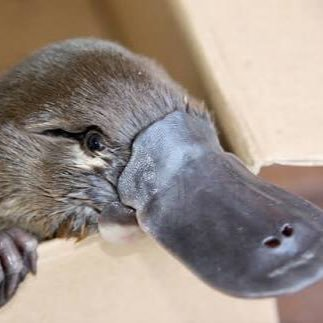
\includegraphics[width=\linewidth]{Platypus.jpg}
\caption{Who's a good boy?}\label{fig:fuzzyduck}
\end{wrapfigure}
\blindtext

\endgroup

\section*{Spacing}
\LaTeX\
Just random \\
The second line is indented. If we   use    multiple spaces
\\[10pt]

% \usepackage{parskip} - include up top


Special Characters
\% \$ \& \_ \textbackslash


\section[Smoothie]{Smoothie Recipe}
\begin{itemize}
\item 1 Cup Spinach
\item 1 Cup Frozen Blueberries
\item 2 Bananas
\item 1.5 Cups Almond Milk
\item Powders
\begin{itemize}
\item 1 Tbs PB2
\item 1 Tsp Ambla Powder
\end{itemize}
\item 6 Dates
\end{itemize}

\setlist{nolistsep}

%\section{Smoothie}
%\blindtext[2]
%\newpage


\section{Perfect Meal Recipe}
\begin{enumerate}[label=\Roman*,font=\bfseries]
\item Add the following and coof for 2 minutes
\begin{itemize}
\item 1 tsp Olive Oil
\item 1 Cup Onion, diced
\item 3 cloves Garlic, minced
\item 1 tsp Salt
\item 1 Cup choppet portobello Mushrooms
\end{itemize}
\item Add the following and cook for 2 minutes
\end{enumerate}

\bigskip

\begin{description}
\item[Platypus] A cute little duck beaver
\item[Bee] Makes delicious honey
\item[Wasp] Basically an asshole with wings.
\end{description}

\begin{tabbing}
Customer \= Name \hspace*{1.5cm}\= Street \hspace*{1.5cm} \=
City \\
\>Viktor Ramses \> 123 Main St \> London \\
\end{tabbing}

\begin{table}
\begin{tabular}{l|l|l}
\textbf{Name} & \textbf{Command} & \textbf{Sample Text} \\
\hline
emphasize & \verb|\emph| & \emph{abcdefgh} \\
italic & \verb|\textit| & \textit{abcdefgh} \\
%slanted & \verb|\textbf| & \textbf{abcdefgh} \\
bold & \verb|\textbf| & \textbf{abcdefgh} \\
small capped & \verb|\textsc| & \textsc{abcdefgh} \\
medium & \verb|\textmd| & \textmd{abcdefgh} \\
upright & \verb|\textup| & \textup{abcdefgh} \\
roman family & \verb|\textrm| & \textrm{abcdefgh} \\
sans serif & \verb|\textsf| & \textsf{abcdefgh} \\
typewriter & \verb|\texttt| & \texttt{abcdefgh} \\
combo & \verb|\textup{textup{\textbf{}}| & \textit{\textbf{abcdefgh}} \\
\end{tabular}
\caption{Ways to emphasize text.}\label{sec:typeemp}

\'{a} \^{e} \`{o} \"{u} \.{a} \={o} \~{n} \u{a} \H{a} \v{e} \t{oo} \c{c} \d{n} \b{i}

ß

\begin{tabular}{@{}*3l@{}}
\multicolumn{2}{c}{Name} &
\multicolumn{1}{c}{Age}\\
First & Last & \\
\hline
Will & Cole & 36\\
Jen & Leadbetter & 39\\
\end{tabular}\\

\end{table}
\begin{figure}[ht]
\centering

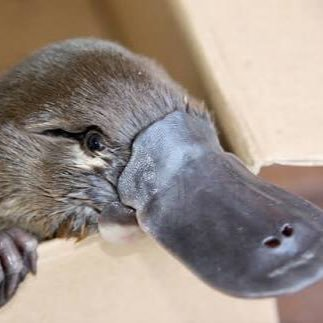
\includegraphics[width=8cm]{Platypus.jpg}
\end{figure}
\blindtext[2]

\section[Type]{\textsf{Type Emphasis \& Sizing}}
\label{sec:typeemp}
\itshape italic, \slshape slanted, \scshape small caps, \upshape upright, \normalfont back to normal\\

Get Smaller : \normalsize{normal}, \small{small}, \footnotesize{footnote}, \scriptsize{script}, \tiny{tiny}

Get Bigger : \large{large}, \Large{larger}, \LARGE{larger}, \huge{huge}, \Huge{Hugest}

\begin{LARGE}
I'm Not Shouting!  This is Just the Way I Talk!!!
\end{LARGE}

\normalsize{This is fine.  Everything is fine.}

\section{\textsf{Font Families}}
We can {\sffamily temporarily change} a font family, \ttfamily or change it for the rest of the document \sffamily

\begin{quote}
"Maybe when our heroes fail us, it's our turn to wear the cape." \\
- Lawrence Meyer
\end{quote}


\section{Math Formulas}
\begin{flalign*}
	& ax^2 + bx + c = 0 &\\
\end{flalign*}

This \( ax^2 + bx + c = 0\) is the quadratic equation. \\

$x=\frac{-b\pm\sqrt{b^2-4ac}}{2a}$ \\
Greek letters $\alpha \beta \gamma \delta \epsilon \zeta \eta \theta \vartheta \iota \kappa \lambda \Lambda
\mu \nu \xi \Xi \pi \Pi \rho \varrho \sigma \Sigma \tau \upsilon \Upsilon \phi \varphi \pi \Pi \chi \psi \Psi \Omega \omega $ \\

Scrpt letters $\mathcal{A}, \mathcal{B}$

Subscript $t_0$ \\

Superscript $x^2$ \\

Operators $\arccos, \arcsin, \arctan, \arg, \cos, \cosh, \cot, \coth, \deg, \det, \dim, \exp, \gcd,\\ \hom, \inf, \ker, \lim, \lg, \liminf, \limsup, \ln, \log,
\max, \min, \Pr, \sec, \sin, \sinh, \sup, \tan, \tanh$ \\

Arrows $\leftarrow, \Leftarrow, \rightarrow, \Rightarrow, \leftrightarrow, \rightleftharpoons, \uparrow, \downarrow, \Uparrow, \Downarrow,
\Leftrightarrow, \Updownarrow, \mapsto, \longmapsto, \nearrow, \searrow, \swarrow, \nwarrow, \leftharpoonup, \rightharpoonup,
\leftharpoondown, \rightharpoondown$ \\

Relational Operators $ \geq, \gg, \leq, \ll, \neq $ \\

Binary Operation/Relation Symbols $ \approx, \asymp, \bowtie, \cong, \dashv, \doteq, \equiv, \frown, \mid, \models, \parallel, \perp, \prec, \preceq,
\propto, \sim, \simeq, \smile, \succ, \succeq, \vdash $ \\

Vectors $\vec{a}\cdot\hat{x}=a_x$ \\

Matrices
$\begin{pmatrix}
1 & 2 \\
3 & 4
\end{pmatrix}$\\
\\
$I_3 =
\begin{pmatrix}
1 & 0 & 0 \\
0 & 1 & 0 \\
0 & 0 & 1
\end{pmatrix}$ \\

Integrals $\Delta x=\int_{t_0}^{t_1}v(t)dt$ \\

Limits $\lim_{x\to0} \frac 1 x = \infty$ \\

Summations $e^x=\sum_{n=0}^\infty\frac{x^n}{n!}$ \\


\section{\textsf{Custom Commands}}

\NTT\ or \NTTB\

Style to \typew{typewriter}.

\section{Text Columns}
{\centering
Get in the middle of me \\
Okay\\[10pt]
}

\quad\parbox{4cm}{I used to think I was indecisive, but then I took an arrow to the knee.}
\quad\parbox{2cm}{Don't forget that you're here for\-ev\-er.}
\quad\parbox{2cm}{\raggedright They say dress for the job you want.  That's why I'm naked.}
\quad\parbox{2cm}{\raggedleft I've decided I don't want children. Too many calories.}

\begin{minipage}{5cm}
Sometimes when you stare into the void, the void gets really uncomfortable and calls HR.
\end{minipage}

\section{Referencing}
You have two wolves inside of you, and this is a problem, because the recommended number of wolves that should be inside a person is zero.
\footnote[2]{Some Internet Rando} \\[5pt]

There is a great table on Type Emphasis in this section~\ref{sec:typeemp} on page~\pageref{sec:typeemp}\\[2pt]

page~\pageref{fig:fuzzyduck}\\[2pt]

How I learned to Stop Worrying and Love the One Ring of Power \cite{ABCLOTR}.

When God gives you lemons it's time to \textsc{\textbf{find a new god}}
{\index{Power}Power Thirst} \\[2pt]

\blindtext

\clearpage
\addcontentsline{toc}{chapter}{index}
\printindex

\begin{thebibliography}{books}
\bibitem{ABCLOTR} J.R.R. Kubrick \emph{The Crustacian Collection}, 1947
\end{thebibliography}

\end{document}